
\begin{figure}[t]
    \centering
    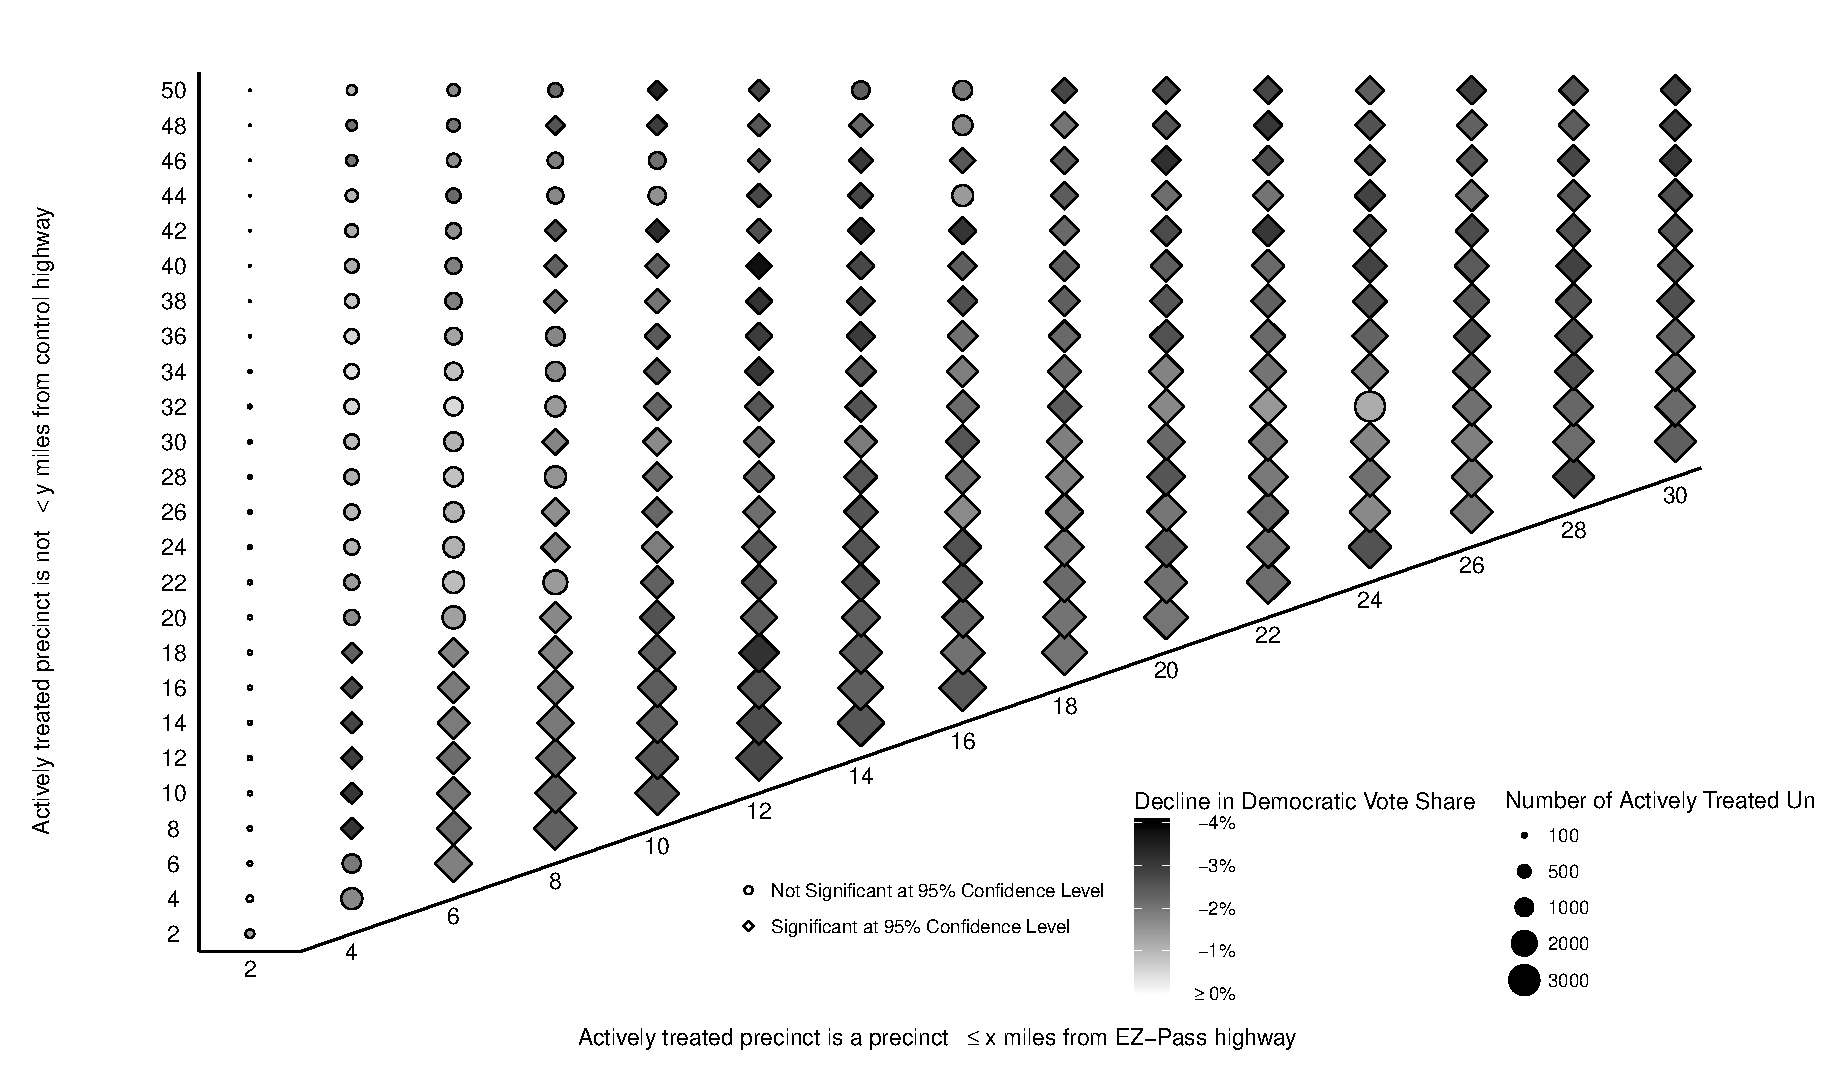
\includegraphics[width=0.9\textwidth]{Figures/new_style_04.eps}
    \label{fig:heatmap}
    \caption{Sensitivity Analysis. X-Y position gives the conditional difference in difference for a given combination of inclusion rule and exclusion rule. For example, at (12,18), one sees the effect of saying treated precincts are those within 12 miles of an EZ-Pass highway but more than 18 miles from a non EZ-Pass highway, and similarly for control units. Effect size is indicated by the darkness of the shape, number of matched units is indicated by the area of the point, and results that are significant at the conventional 95\% threshhold are indicated by diamonds. Generally, effect magnitudes and significance are not sensitive to choice of rule, changes in effect magnitude are gradual.}
\end{figure}